\documentclass{article}
\usepackage[top=1in, bottom=1in, left=1in, right=1in]{geometry}
% \usepackage{fullpage, fancyhdr}
\usepackage{fullpage}
\usepackage{float}
\usepackage{mathtools}
\usepackage{caption}
\usepackage{sidecap} % enable side captions
\usepackage{subcaption}
\usepackage{portland}
\usepackage{graphicx}
\setlength{\topmargin}{0.0in}
\setlength{\headheight}{0.5in}
\setlength{\headsep}{0in}
\setlength{\footskip}{9pt}

% General tikz + pgf-umlsd
\usepackage{wrapfig}
\usepackage{listings}
\usepackage{tikz}
\usepackage{pgf-umlsd}
\usepgflibrary{arrows}
\usetikzlibrary{shapes,arrows,shadows}
% \usepackage[english]{babel} % Include this to prevent tikz-uml from hic-cuping on nested umlcall's. 


\DeclareMathAlphabet{\mathpzc}{OT1}{pzc}{m}{it}
\newcommand{\z}{\mathpzc{z}}

% Use so that included code is pretty
\usepackage{listings}
\usepackage{color}

\definecolor{dkgreen}{rgb}{0,0.6,0}
\definecolor{gray}{rgb}{0.5,0.5,0.5}
\definecolor{mauve}{rgb}{0.58,0,0.82}

\lstset{ %
  backgroundcolor=\color{white},  % choose the background color; you must add \usepackage{color} or \usepackage{xcolor}
  basicstyle=\footnotesize,       % the size of the fonts that are used for the code
  breakatwhitespace=false,        % sets if automatic breaks should only happen at whitespace
  breaklines=true,                % sets automatic line breaking
  captionpos=t,                   % sets the caption-position to bottom
  commentstyle=\color{dkgreen},   % comment style
%   deletekeywords={...},           % if you want to delete keywords from the given language
%   escapeinside={\%*}{*)},         % if you want to add LaTeX within your code
%   extendedchar=false,             % lets you use non-ASCII characters; for 8-bits encodings only, does not work with UTF-8
  frame=single,                   % adds a frame around the code
  keywordstyle=\color{blue},      % keyword style
  language={[x86masm]Assembler},                % the language of the code
  morekeywords={LDR,AREA,ENTRY,CODE,DATA,DCD,SPACE,BLT,B,BL.W,ADDS,VMOV,IN,ZAP,MAC,APAC,ADD,SACH,MACD,OUT,},           % if you want to add more keywords to the set
  numbers=left,                   % where to put the line-numbers; possible values are (none, left, right)
  numbersep=5pt,                  % how far the line-numbers are from the code
  numberstyle=\tiny\color{gray},  % the style that is used for the line-numbers
  rulecolor=\color{black},        % if not set, the frame-color may be changed on line-breaks within not-black text (e.g. comments (green here))
  showspaces=false,               % show spaces everywhere adding particular underscores; it overrides 'showstringspaces'
  showstringspaces=false,         % underline spaces within strings only
  showtabs=false,                 % show tabs within strings adding particular underscores
  stepnumber=1,                   % the step between two line-numbers. If it's 1, each line will be numbered
  stringstyle=\color{mauve},      % string literal style
  tabsize=8,                      % sets default tabsize to 2 spaces
  title=\lstname                  % show the filename of files included with \lstinputlisting; also try caption instead of title
}



% \pagestyle{fancyplain}
\pagestyle{myheadings}
\voffset=-0.50in
\topmargin=0.00in 
\headsep=0.25in 
\evensidemargin=0in 
\oddsidemargin=0in 
\textwidth=6.6in 
\textheight=10.0in 

\renewcommand{\topfraction}{0.9}	% max fraction of floats at top
\renewcommand{\bottomfraction}{0.8}	% max fraction of floats at bottom
%   Parameters for TEXT pages (not float pages):
\setcounter{topnumber}{2}
\setcounter{bottomnumber}{2}
\setcounter{totalnumber}{4}     % 2 may work better
\setcounter{dbltopnumber}{2}    % for 2-column pages
\renewcommand{\dbltopfraction}{0.9}	% fit big float above 2-col. text
\renewcommand{\textfraction}{0.07}	% allow minimal text w. figs
%   Parameters for FLOAT pages (not text pages):
\renewcommand{\floatpagefraction}{0.7}	% require fuller float pages
% N.B.: floatpagefraction MUST be less than topfraction !!
\renewcommand{\dblfloatpagefraction}{0.7}	% require fuller float pages
% remember to use [htp] or [htpb] for placement

\title{Assignment \# 7: Problem Set 4, Problem 2}
\date{2/15/2013}
\author{Brian Arnberg}

\markright{Brian Arnberg\hfill ELEC 6260 - Embedded Computing Systems\hfill}     
\setlength{\parindent}{0pt}


\renewcommand{\figurename}{\bf Q3 -}


\begin{document}\label{start}

\tikzstyle{endpoint} = [circle, draw, text width=1.8em, text centered, rounded corners, minimum height=1.8em]
\tikzstyle{block} = [rectangle, draw, text width=12.3em, text centered, rounded corners, minimum height=2em]
\tikzstyle{decision} = [diamond, draw, text width=4.5em, text badly centered, node distance=1.9cm, inner sep=0pt]
\tikzstyle{line} = [draw, -latex']

% \begin{titlepage}
	\maketitle
	\thispagestyle{empty}
% \end{titlepage}

% \section*{Assignment \# 7: Problem Set 4, Problem 2 - Due 2/15/2013}
At the end of Chapter 3, answer/work the following, which deal with input/output operations:\\
Q3-6, Q3-8, Q3-9, Q3-12, Q3-12, Q3-13, Q3-15, Q3-16, Q3-19.

% -----------------------------------------------%
% ---------   Q3-6   ----------------------------%      
\setcounter{figure}{5}
\begin{figure}[h]
	\centering
\caption{Draw a UML sequence diagram for a busy-wait read of a device. The diagram should include the program running on the CPU and the device.}
\begin{sequencediagram}
	\newthread{c}{:CPU}
	\newinst[1]{p}{:PollDevice}
	\newthread{d}{:Device}
	\begin{sdblock}{Main Loop}{}
		\begin{call}{c}{poll()}{p}{ready}
			\begin{sdblock}{Wait for Device}{}
				\mess{d}{Ready()}{p}
			\end{sdblock}
		\end{call}
	\begin{call}{c}{read()}{d}{value}
	\end{call}
	\end{sdblock}
\end{sequencediagram}
\end{figure}

% -----------------------------------------------%
% ---------   Q3-8   ----------------------------%      
\setcounter{figure}{7}
\begin{figure}[th]
\centering
\caption{Draw a UML sequence diagram for copying characters from an input to an output device using busy-wait I/O. The diagram should include the two devices and the two busy-wait I/O handlers.}
\begin{sequencediagram}
	\newthread{f}{:Foreground}
	\newinst[1]{ih}{:InputHandler}
	\newthread{id}{:InputDevice}
	\newinst[1]{oh}{:OutputHandler}
	\newthread{od}{:OutputDevice}
	\begin{sdblock}{Main Loop}{}
		\begin{call}{f}{getChar()}{ih}{char}
			\begin{sdblock}{Wait for Device}{} 
				\mess{id}{InputReady()}{ih}
			\end{sdblock}
			\begin{call}{ih}{ReadInput()}{id}{char}
			\end{call}
		\end{call}
		\begin{call}{f}{writeChar()}{oh}{}
			\begin{sdblock}{Wait for Device}{}
				\mess{od}{OutputReady()}{oh}
			\end{sdblock}
			\begin{call}{oh}{writeOutput()}{od}{}
			\end{call}
		\end{call}
	\end{sdblock}
\end{sequencediagram}
\end{figure}

% -----------------------------------------------%
% ---------   Q3-9   ----------------------------%      
\setcounter{figure}{8}
\begin{figure}[h]
	\centering
	\caption{When would you prefer to use busy-wait I/O over interrupt driven I/O?\\
	\emph{Answer:} One would prefer busy-wait I/O over interrupt driven I/O in situations wherein the main program cannot function until a device is ready to service. For instance, a calculator should wait for user input before it does anything, and once it has calculated (and displayed) the output, it should wait for more user input.  }
\end{figure}

% -----------------------------------------------%
% ---------   Q3-12  ----------------------------%      
\setcounter{figure}{11}
\begin{figure}[h]
	\centering
	\caption{Draw a UML sequence diagram for an interrupt-driven write of a device. The diagram should include the background program, the handler, and the device.}
\begin{sequencediagram}
	\newthread{c}{:CPU}
	\newinst[2]{b}{:Background}
	\newinst[1]{i}{:Interrupt Handler}
	\newthread{d}{:Device}
	\begin{call}{c}{Background}{b}{Save Contex}
		\mess{d}{Interrupt}{c}
		\begin{callself}{c}{Determine Source}{}
		\end{callself}
	\end{call}
	\begin{call}{c}{Process Interrupt}{i}{Restore Context}
		\begin{call}{i}{Write}{d}{}
		\end{call}
	\end{call}
	\begin{messcall}{c}{Return to Background}{b}
	\end{messcall}
\end{sequencediagram}

\end{figure}

% -----------------------------------------------%
% ---------   Q3-13  ----------------------------%      
\setcounter{figure}{12}
\begin{figure}[h]
	\centering
	\caption{Draw a UML sequency diagram for a vectored interrupt-driven read of a device. The diagram should include the background program, the interrupt vector table, the handler, and the device.}
\begin{sequencediagram}
	\newthread{c}{:CPU}
	\newinst[2]{b}{:Background}
	\newinst{v}{:Interrupt Vectors}
	\newinst{i}{:Interrupt Handler}
	\newthread{d}{:Device}
	\begin{call}{c}{Background}{b}{Save Current Context}
		\mess{d}{Interrupt}{c}
		\begin{callself}{c}{Determine Source}{}
		\end{callself}
	\end{call}
	\begin{call}{c}{Get Interrupt Vector}{v}{Vector}
	\end{call}
	\begin{call}{c}{Process Interrupt}{i}{Restore Context}
		\begin{call}{i}{Read}{d}{}
		\end{call}
	\end{call}
	\begin{messcall}{c}{Return to Background}{b}
	\end{messcall}

\end{sequencediagram}
\end{figure}


% -----------------------------------------------%
% ---------   Q3-15  ----------------------------%      
\setcounter{figure}{14}
\begin{figure}[h]
	\centering
	\caption{Draw a UML sequence diagram of a higher-priority interrupt that happens during a lower-priority interrupt handler. The diagram should include the device, the two handlers, and the background program.} 
\begin{sequencediagram}	
	\newthread{c}{:CPU}
	\newinst[2]{b}{:Background}
	\newinst{i1}{:Handler 1 (Higher Priority)}
	\newinst{i2}{:Handler 2}
	\newthread{d}{:Device}

	\begin{messcall}{c}{Background}{b}{}
		\mess{d}{Interrupt 2}{c}
		\begin{callself}{c}{Determine Source}{2}
		\end{callself}
		\begin{callself}{c}{Save Context}{}
		\end{callself}
	\end{messcall}

	\begin{messcall}{c}{Handle Interrupt 2}{i2}{}
		\begin{callself}{i2}{Start}{}
		\end{callself}
		\mess{d}{Interrupt 1}{c}
		\begin{callself}{c}{Determine Source}{1}
		\end{callself}
		\begin{callself}{c}{Save Context}{}
		\end{callself}
	\end{messcall}

	\begin{call}{c}{Handle Interrupt 1}{i1}{Restore Context}
		\begin{callself}{i1}{Execute Everything}{}
		\end{callself}
	\end{call}

	\begin{call}{c}{Return to Interrupt 2}{i2}{Restore Context}
		\begin{callself}{i2}{Finish}{}
		\end{callself}
	\end{call}

	\begin{messcall}{c}{Return to Background}{b}
	\end{messcall}
\end{sequencediagram}	
\end{figure}

% -----------------------------------------------%
% ---------   Q3-16  ----------------------------%      
\setcounter{figure}{15}
\begin{figure}[h]
	\centering
	\caption{Draw a UML sequence diagram of a lower-priority interrupt that happens during a higher-priority interrupt handler. The diagram should include the device, the two handlers, and the background program.} 
\begin{sequencediagram}	
	\newthread{c}{:CPU}
	\newinst[2]{b}{:Background}
	\newinst{i1}{:Handler 1 (Higher Priority)}
	\newinst{i2}{:Handler 2}
	\newthread{d}{:Device}

	\begin{messcall}{c}{Background}{b}{}
		\mess{d}{Interrupt 1}{c}
		\begin{callself}{c}{Determine Source}{1}
		\end{callself}
		\begin{callself}{c}{Save Context}{}
		\end{callself}
	\end{messcall}

	\begin{call}{c}{Handle Interrupt 1}{i1}{Restore Context}
		\begin{callself}{i1}{Start}{}
		\end{callself}
		\mess{d}{Interrupt 2}{c}
		\begin{callself}{c}{Determine Source}{2}
		\end{callself}
		\begin{callself}{i1}{Finish}{}
		\end{callself}
	\end{call}

	\begin{call}{c}{Handle Interrupt 2}{i2}{Restore Context}
		\begin{callself}{i2}{Execute Everything}{}
		\end{callself}
	\end{call}

	\begin{messcall}{c}{Return to Background}{b}
	\end{messcall}
\end{sequencediagram}	
\end{figure}


% -----------------------------------------------%
\newpage
% ---------   Q3-19  ----------------------------%      
\setcounter{figure}{18}

\begin{figure}[h]
	\centering
	\caption{Three devices are attached to a microprocessor: Device 1 has highest priority and device 3 has lowest priority. Each device's interrupt handler takes 5 time unites to execute. Show what interrupt handler (if any) is executing at each time given the sequency of device interrupts displayed below.}
	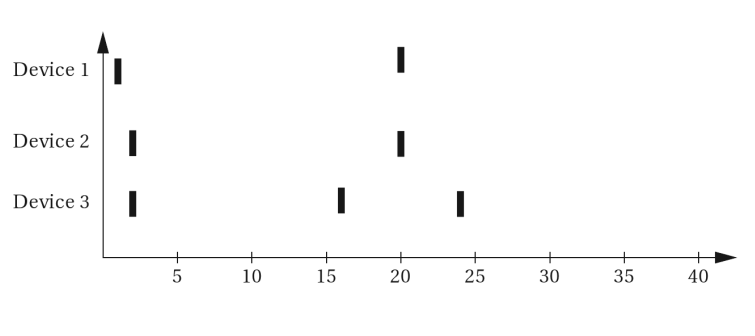
\includegraphics[width=\textwidth,keepaspectratio]{Q3-19}
\end{figure}

% -----------------------------------------------%
%  \begin{figure}[htbp]
%   \centering
%   \includegraphics[width=4.0in,keepaspectratio]{E-Field}
%   \caption{\small{ The E-Field pattern produced by the initial code. }}
%   \label{fig:E-Field}
%   \end{figure}
%  \begin{figure}[htbp]
%   \centering
%   \includegraphics[width=4.0in,keepaspectratio]{Power}
%   \caption{\small{ The normalized power pattern of the system.  }}
%   \label{fig:Power}
%   \end{figure}

\label{end}\end{document}


